\section{Driving forces and fluxes for diffusion}

We know how materials are formed by atoms placed in symmetric positions in space in order to form an ordered lattice, but this is entirely true only in theory. In fact, real materials present a large series of defects, wanted and unwanted, that locally destroy the symmetry and change materials properties. One of the most important types of defects that exist are impurities, where atoms of types different from the ones of the normal materials are present inside the structure. In particular, we want to focus on the situation where those atoms are smaller than the principle one having so that they enter interstitial sites where they can move between larger atoms, like in \figref{fig:Inter}.
\begin{figure}[b]
    \centering
    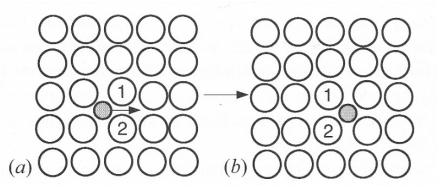
\includegraphics[width=0.8\textwidth]{Immagini/Inter.png}
    \caption
    {
        Example of diffusion of an interstitial atom inside a general simple lattice.
    }
    \label{fig:Inter}
\end{figure}
A practical example of such a phenomenon is the diffusion of Carbon inside Iron, or Hydrogen in a general material. Such movements are able to give the material particular properties or drive it to different equilibrium respect the one we imagine. Therefore, we want to focus on the study of atoms movements inside the material to create a good model for diffusion processes to then apply them into material modelling.

In order to do that we shall focus on the description of the flux of particles of $i$-th type, $\vb{J}_i$, inside the material, and we have seen that is related to the gradient of chemical potential. Still, we can see more in depth how they are related by defining a really important quantity called \textbf{mobility} as follows.
\dfn{Mobility}
{
    The mobility of atoms of type $i$, $M_i$, inside a material is constant of proportionality between the average particle velocity and the gradient of chemical potential
    \begin{equation}
        \left\langle \vb{v}_i \right\rangle = -M_i\grad \mu_i.
    \end{equation}
}
\noindent
Then, from this definition one can easily see how the flux and chemical potential are related since $\vb{J}_i$ is given by the density of that type of atoms $c_i$ multiplied by the average velocity, having
\begin{equation}
    \label{eq:fluxForm}
    \vb{J}_i = c_i \left\langle \vb{v}_i \right\rangle = -c_iM_i\grad \mu_i.
\end{equation}
Which is the relation we have seen in the previous part when talking about the $\mathcal{L}$ matrix. Still, we can work the expression a little more and see how in reality we can collect the flux at the gradient of concentration using the following result.
\thm{Fick's law}
{
    Inside a material, if the interstitial moving atoms are much less compared to the solvent atoms so that the system can be approximated to a dilute solution we can write the flux of atoms as
    \begin{equation}
        \vb{J}_i = -k_B TM_i\grad c_i = -D_i\grad c_i,
    \end{equation}
    where $D_i$ is also called \textbf{diffusion constant}.
}
\pf{Proof}
{
    Since the system can be thought of a dilute solution the Henry’s law can be used so that the chemical potential is
    \begin{equation}
        \mu_i = \mu_i^0 + k_BT\ln\left( \gamma_i^0X_i \right) = \mu_i^0 + k_BT\ln\left( \gamma_i^0\frac{N_i}{V}\frac{V}{N_T} \right) = \mu_i^0 + k_BT\left[ \ln\left( \frac{\gamma_i^0}{\left\langle c \right\rangle} \right) + \ln c_i\right].
    \end{equation}
    We can see how in this relation $\gamma_i^0/\left\langle c \right\rangle$ is a constant, so that by taking the gradient we have that a relation between $\mu_i$ and $c_i$ is obtained as
    \begin{equation}
        \grad \mu_i = \frac{k_BT}{c_i}\grad c_i.
    \end{equation}
    Then by substituting it inside \eqref{eq:fluxForm} the wanted relation is obtained, with also the important equality
    \begin{equation}
        D_i = k_BTM_i,
    \end{equation}
    which is also called \textbf{Nernst-Einstein relation}.
}

\subsection{Vacancies in equilibrium}

As we have said a lot of different type of defects can be present inside solids, citing principally substitutional defects, but another important type that allows for diffusion to appear are vacancies. The latter is non-other than the absence of one atom in a ceratin position and are able to variate the band structure of the material along with also diffuision properties. For this reason is interesting to see how effectively they appear, in particular it's possible to give an estimate of the molar fraction of vacancies inside a material in equilibrium by using the following result.
\thm{Vecancy presence}
{
    In a material coposed by $N_A$ atoms and $N_V$ vacancies, if we have $N_V \ll N_A$, we have that at equilibrium the molar fraction of vacancies is
    \begin{equation}
        X_V = \exp\left( -\frac{G_V^f}{k_BT} \right) = \exp\left( \frac{S_V^f}{k_B} \right)\exp\left( -\frac{H_V^f}{k_BT} \right),
    \end{equation} 
    where $G_V^f$ is the varation of free energy needed in order to form the vacancy in the cristal.
}
\pf{Proof}
{
    We can write down the free energy of the system by adding to the free enrgy of the single component the increase of entropy given by using Bragg-Williams-Gorsky configurational entropy once again, and having
    \begin{equation}
        G = N_A\mu_A^0 + N_V G_V^f + k_BT\left[ N_A\ln\left( \frac{N_A}{N_A + N_V} \right) + N_V\ln\left( \frac{N_V}{N_A + N_V} \right) \right].
    \end{equation}
    From this we use the fact that $N_V \ll N_A$ and evaluate the chemical potentials of the two components having
    \begin{align}
        &\mu_A = \pdv{G}{N_A} \approx \mu_A^0, &\mu_V = \pdv{G}{N_V} \approx G_V^f + k_BT\ln X_V.
    \end{align}
    At equilibirum we need $\partial G/\partial N_V = 0$ meaning that we can obtain the wanted relation by simply setting $\mu_V = 0$ and inverting it.
}
\noindent
It's interesting becouse the value of $X_V$ can be experimentally measured by differential difrattometry at different temperatures, where the variation of the volume can be obtained and then the one that comes from thermal expansion can be omited by evaluating the lattice constatn using diffraction. Still, $X_V$ can be computed and so by doing a logarithmic fit one can obtain the value fo $H_V^f$ which can be useful for some other investigations, also the general values are around \SI{0.65}{\electronvolt}.